%
% Web Cryptography API
% @author Pieter Maene <pieter.maene@student.kuleuven.be>
%

\section{Future Work: Web Cryptography API}
\label{sec:web_cryptography_api}

Currently, web developers implement cryptographic functionality in JavaScript. Despite great improvements in recent years, it is still slower than native code.\cite{site:resig_javascript_performance_rundown}\cite{site:cois_javascript_performance_rundown_2012}\cite{smedberg_performance_analysis_of_javascript} In 2012 a working group was started by W3C to write the Web Cryptography API specification, which would add cryptographic functionality to user agents.\cite{wiki:webcrypto} The specification defines the \texttt{SubtleCrypto} interface which has several high-level functions.\cite{sleevi_watson_web_cryptography_api} There are methods to manage the keys and to encrypt data. The API only supports a specific set of algorithms, nor does each algorithm support all functions of the interface.

\par Since the specification has not been completed yet, most user agents do not support it. Internet Explorer 11 is the only browser that already has an implementation, but it misses some algorithms.\cite{site:microsoft_web_cryptography} Therefore, the NfWebCrypto polyfill was used for the benchmarks. This is a \cplusplus plugin for Chrome, so its performance should be comparable to a real implementation. Since a polyfill had to be used, the API's functionality was not yet added to Helios.

\subsection{Modular Exponentation}
\label{sec:wc:modular_exponentiation}

Helios uses ElGamal to encrypt the ballots, which is an algorithm not supported by the API. The modular exponentiations are responsible for the majority of the calculation time. An improvement there would impact overall performance.

\par Since the API only offers high-level functions, this had to be implemented separately. Diffie-Hellman is one of the supported algorithms. The \texttt{deriveKey} method uses \ref{eq:wc:diffie_hellman} to calculate the shared secret.\cite{diffie_hellman_new_directions_in_cryptography}

\begin{equation}
  \label{eq:wc:diffie_hellman}
  K = (g^a)^b \mod{p}
\end{equation}

\par In this equation, $g^a$ is the public key of A and $b$ the private key of B. If the public and private key can be specified, it can be used to calculate the modular exponentiation $x^y \mod{p}$. It is possible to import a specific private key into the user agent's key store. For the Diffie-Hellman algorithm, the specification only allows private keys in the PCKS8 format to be imported. To make testing easier, the NfWebCrypto plugin was modified to allow the import of raw keys. After calculating the shared secret, the result can be obtained with the \texttt{exportKey} function.

\par The performance of the NfWebCrypto library is compared to that of JSBN and Leemon, two JavaScript big number libraries.\cite{site:wu_rsa_and_ecc_in_javascript}\cite{site:baird_big_integers_in_javascript} A \np{1024}-bit exponent is used, which is the size of the keys used by Helios. The calculation is repeated \np{1000} times for each library. The results are shown in \ref{fig:wc:modular_exponentiation} and \ref{tab:wc:modular_exponentiation}. The first exponentiation of the NfWebCrypto plugin took a lot longer, which explains the large variance. The NfWebCrypto plugin result was not correct. The communication with the plugin has to be \texttt{base64} encoded, which resulted in conversion issues between \cplusplus and JavaScript.

\begin{figure}
  \centering
  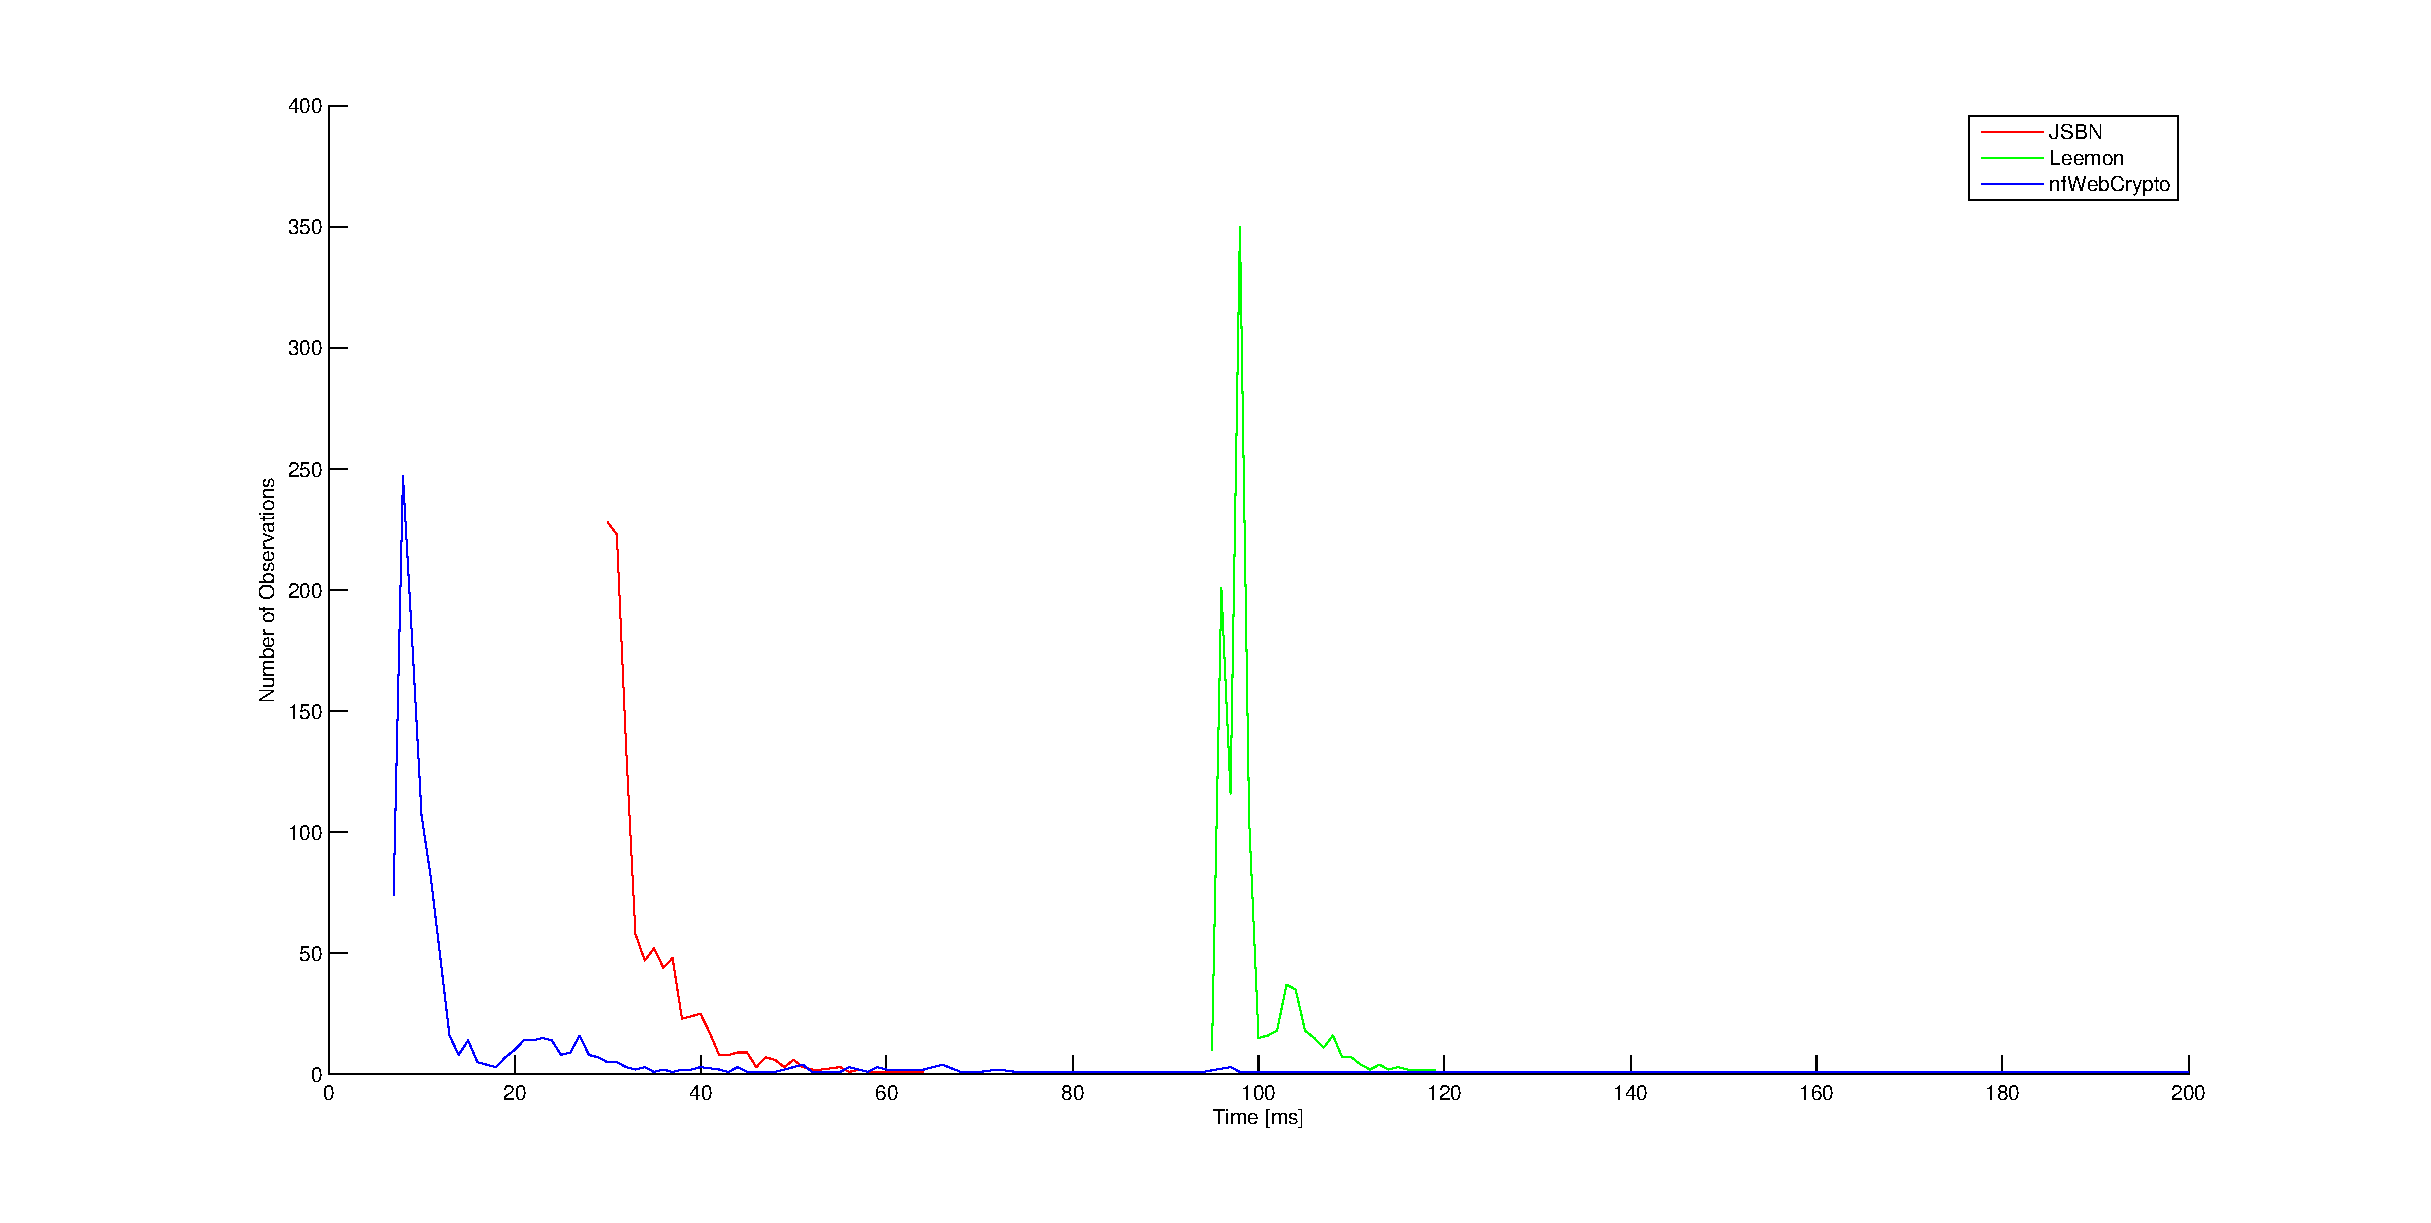
\includegraphics[width=\linewidth]{modular_exponentiation.eps}
  \caption{Modular Exponentiation}
  \label{fig:wc:modular_exponentiation}
\end{figure}

\begin{table}
  \centering
  \caption{Modular Exponentiation}
  \label{tab:wc:modular_exponentiation}
  \begin{tabular}{r | c c}
    Library & Average [ms] & Variance [ms] \\ \hline
    JSBN & 33.9250 & 26.5019  \\
    Leemon & 99.1470 & 15.0785 \\
    NfWebCrypto & 16.0670 & 470.6251
  \end{tabular}
\end{table}

\subsection{RSA}

RSA was used to make a second comparison between JSBN and NfWebCrypto. This cipher isn't used by Helios, but the results are very interesting. A standard value of \np{65537} was used for the public exponent of the encryption. Notice that this is a lot shorter than the exponents used in \ref{sec:wc:modular_exponentiation}. The modulus is \np{1024} bits large.

\par JSBN has specific functions for RSA encryption and decryption. The Web Cryptography API supports the \texttt{RSAES-PKCS1-v1\_5} algorithm.\cite{rfc3447} Although public keys in the SPKI format can be imported, this proved difficult. Therefore, a new key was generated for each encryption. The time required for this is not taken into account. The results are shown in \ref{fig:wc:rsa} and \ref{tab:wc:rsa}. Surprisingly, the JavaScript implementation is faster than the NfWebCrypto plugin. This is caused by communication overhead.

\begin{figure}
  \centering
  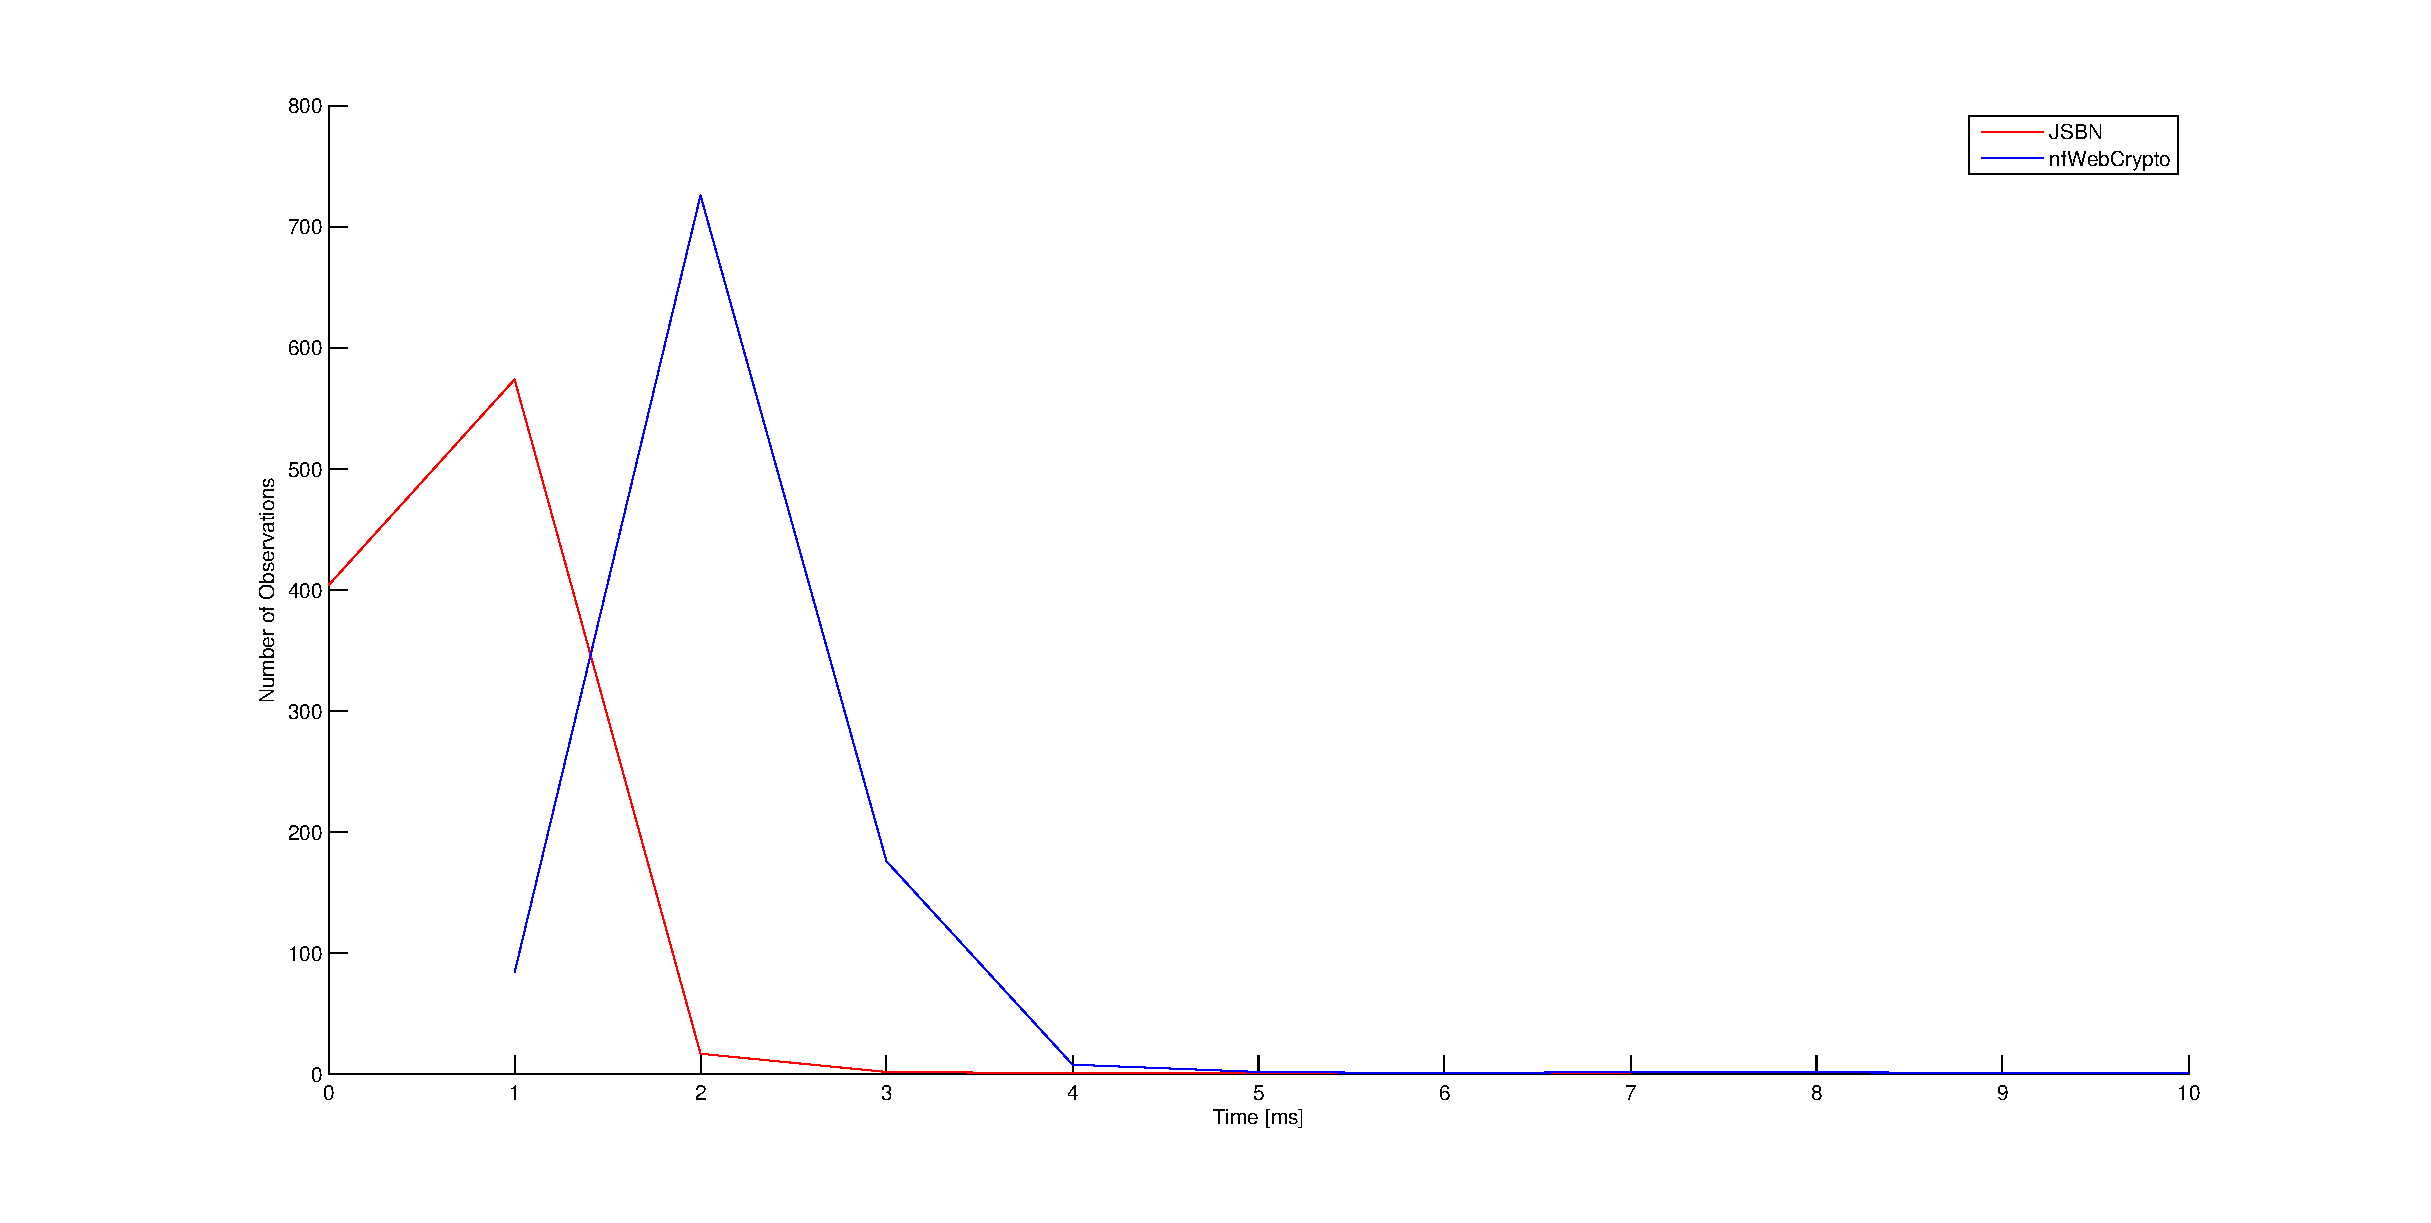
\includegraphics[width=\linewidth]{rsa.eps}
  \caption{RSA}
  \label{fig:wc:rsa}
\end{figure}

\begin{table}
  \centering
  \caption{RSA}
  \label{tab:wc:rsa}
  \begin{tabular}{r | c c}
    Library & Average [ms] & Variance [ms] \\ \hline
    JSBN & 0.6310 & 0.3632  \\
    NfWebCrypto & 2.1360 & 0.4219
  \end{tabular}
\end{table}